\section{Mosaicity and texture}
Imperfect 2D powders exhibit out-of-plane texture, with crystallite \(c\) axes
distributed about the substrate normal (Fig.~\ref{fig:mosaic}). 



\begin{figure}[!ht]
  \centering
  
\includegraphics[width=0.45\linewidth]{mosaic/mosaic_schematic.png}
  \caption{Schematic of crystallite $c$-axis misorientation (mosaicity). A distribution of crystallite orientations may form in a thin-film.}
  \label{fig:mosaic}
\end{figure}
We describe out-of-plane texture by a misorientation density \(\omega(\Delta\theta)\),
where \(\Delta\theta\) is the tilt relative to the mean \(\theta_0\). We take \(\omega\) to be a
unit-normalized Lorentzian--Gaussian mixture,
\[
\omega(\Delta\theta)=\eta\,\frac{1}{\pi}\frac{\gamma}{\Delta\theta^{2}+\gamma^{2}}
+(1-\eta)\,\frac{1}{\sqrt{2\pi}\sigma}\exp\!\left(-\frac{\Delta\theta^{2}}{2\sigma^{2}}\right),
\qquad 0\le\eta\le 1,
\]
with Lorentzian HWHM \(\gamma\) and Gaussian standard deviation \(\sigma\).
Because \(\Delta\theta\) is defined modulo \(2\pi\), we use the \(2\pi\)-periodic wrapped form
(normalized on \((-\pi,\pi]\); see SI).

For a reflection \(\bm G_{HKL}\) we work in the meridional section \((G_r,G_z)\) with
\(G_r=\sqrt{H^2+K^2}\), \(G_z=L\), and \(R=|\bm G|\). At fixed \(R\), orientations lie on the
Bragg circle \(G_r=R\cos\theta\), \(G_z=R\sin\theta\), with the ideal condition at \(\theta_0\).
Mosaicity redistributes intensity along the circle with line density \(I_0\,\omega(\Delta \theta)\).


% requires: \usepackage{subcaption}

\begin{figure}[!ht]
  \centering

  % --- top row: 2D schematic Bragg-circle views ---
  \begin{subfigure}[t]{0.48\linewidth}
    \centering
    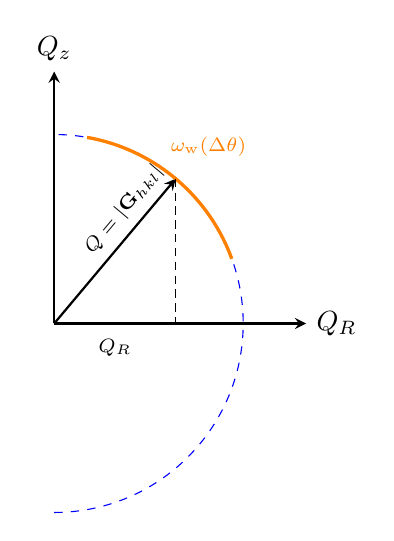
\begin{tikzpicture}[scale=2,>=stealth]
  \def\R{1.2}        % Bragg-sphere radius
  \def\Raxis{1.6}    % axis length
  \def\angleMid{50}  % midpoint angle of mosaic arc (degrees)

  % Folded Bragg locus in the radial coordinate Q_R >= 0
  \draw[dashed,blue] (0,-\R) arc (-90:90:\R);

  % reciprocal-space axes
  \draw[->,thick] (0,0) -- (0,\Raxis) node[above] {$Q_z$};
  \draw[->,thick] (0,0) -- (\Raxis,0) node[right] {$Q_R$};

  % radius vector at midpoint of mosaic arc, label closer to tip
  \coordinate (Gvec) at ({\R*cos(\angleMid)},{\R*sin(\angleMid)});
  \draw[thick,->] (0,0) -- (Gvec)
       node[pos=0.7, above, sloped] {\scriptsize $Q=|\mathbf G_{hkl}|$};

  % mosaic arc on the Bragg sphere, labeled with omega(theta)
  \draw[very thick,orange]
    ({\R*cos(20)},{\R*sin(20)}) arc (20:80:\R)
    node[pos=0.6, above right] {\scriptsize $\omega_{\mathrm w}(\Delta\theta)$};

  % projection onto the radial reciprocal-space axis
  \coordinate (Gr) at ({\R*cos(\angleMid)},0);
  \draw[densely dashed] (Gvec) -- (Gr);
  \node[below, yshift = -2pt] at ({0.5*\R*cos(\angleMid)},0) {\scriptsize $Q_R$};

\end{tikzpicture}

    \caption{In-plane Bragg-circle ($G_r\neq 0$).}
    \label{fig:mosaic_combo:schem_inplane}
  \end{subfigure}\hfill
  \begin{subfigure}[t]{0.48\linewidth}
    \centering
    \begin{tikzpicture}[scale=2,>=stealth]
  \def\R{1.2}
  \def\Raxis{1.6}
  \def\angleMid{90}

  % Folded Bragg locus in the radial coordinate Q_R >= 0
  \draw[dashed,blue] (0,-\R) arc (-90:90:\R);

  % Reciprocal-space axes
  \draw[->,thick] (0,0) -- (0,\Raxis) node[above] {$Q_z$};
  \draw[->,thick] (0,0) -- (\Raxis,0) node[right] {$Q_R$};

  % Specular reciprocal vector
  \coordinate (Gvec) at ({\R*cos(\angleMid)},{\R*sin(\angleMid)});
  \draw[thick,->] (0,0) -- (Gvec)
       node[pos=0.75, right] {\scriptsize $Q=|\mathbf G_{00l}|$};

  % Narrow core near the axis and broad component at larger tilt
  \draw[very thick,oiPurple]
    ({\R*cos(80)},{\R*sin(80)}) arc (80:90:\R)
    node[pos=0.45, above right, text=oiPurple] {\scriptsize narrow core};
  \draw[very thick,oiOrange,dashed]
    ({\R*cos(55)},{\R*sin(55)}) arc (55:80:\R)
    node[pos=0.45, right, text=oiOrange] {\scriptsize broad component};
\end{tikzpicture}

    \caption{Specular Bragg-circle ($G_r=0$.}
    \label{fig:mosaic_combo:schem_specular}
  \end{subfigure}

  \vspace{0.6em}

  % --- bottom row: corresponding detector images ---
  \begin{subfigure}[t]{0.48\linewidth}
    \centering
    
\includegraphics[width=0.85\linewidth]{mosaic/inplane_detector_band.png}
    \caption{In-plane $\omega(\Delta\theta)$ smears into a band upon azimuthal rotation of $\omega(\theta)$.}
    \label{fig:mosaic_combo:img_inplane}
  \end{subfigure}\hfill
  \begin{subfigure}[t]{0.48\linewidth}
    \centering
    
\includegraphics[width=0.85\linewidth]{mosaic/specular_detector_cap.png}
    \caption{Specular $\omega(\Delta\theta)$ rotates to form a cap upon applying $\omega(\theta)$.}
    \label{fig:mosaic_combo:img_specular}
  \end{subfigure}

  \caption{Mosaic broadening viewed in the $\{G_r,G_z\}$ plane (top) and its detector-space manifestation (bottom). Intensity is redistributed along the Bragg circle with line density $I_0\,\omega(\Delta\theta)$: (left) an in-plane condition with $G_r\neq 0$ yields two arcs of reflection, and (right) a specular reflection with $G_r=0$ concentrates intensity near the polar cap, producing a single arc.}
  \label{fig:mosaic_combo}
\end{figure}

Random in-plane rotations about the film normal revolve the meridional line density
about the \(G_z\) axis, generating an axially symmetric distribution on the Bragg sphere.

A latitude ring at polar angle \(\theta\) has area \(dA=2\pi R^{2}\sin\theta\,d\theta\), so
intensity conservation \(I_0\,\omega(\theta-\theta_0)\,d\theta=\sigma(\theta)\,dA\) gives
\begin{equation}
  \sigma(\theta)=\frac{I_0}{2\pi R^2\sin\theta}\,\omega(\theta-\theta_0),
  \qquad 0<\theta<\pi.
  \label{eq:mosaic_sigma_maintext}
\end{equation}

Equation~\eqref{eq:mosaic_sigma_maintext} defines the mosaic kernel used to broaden
ideal Bragg points into caps and rings on the Bragg sphere prior to detector projection.


The reciprocal-space consequences appear on an area detector in
Fig.~\ref{fig:mosaic_pbi2}. Strong out-of-plane texture concentrates specular
intensity near discrete $G_z$ values at $G_r=0$ (region A), while random
in-plane orientation distributes in-plane reflections uniformly in azimuth
about $G_z$, producing ring-like features (region B).

\begin{figure}[!ht]
  \centering
  
\includegraphics[width=0.3\linewidth]{mosaic/pbi2_waxs.png}
  \caption{WAXS pattern of PbI$_2$ at $\theta=4^\circ$. Region A: specular reflections. Region B: in-plane scattering.}
  \label{fig:mosaic_pbi2}
\end{figure}

In the in-plane region (Fig.~\ref{fig:mosaic_pbi2}B), the Ewald sphere intersects the broadened Bragg-sphere feature along an extended band. Azimuthal averaging then produces band-like scattering whose radial width and line shape are set primarily by the core of $\omega$ and by the Jacobian factor $1/\sin\theta$ in Eq.~\eqref{eq:mosaic_sigma_maintext}.

In the specular region (Fig.~\ref{fig:mosaic_pbi2}A), the same kernel produces cap-like broadening about the specular reflections. A specular reflection is satisfied when the scattering condition selects crystallites whose tilt shifts the reflection from $\theta_0$ to $\theta_0+\Delta\theta$. The residual intensity therefore scales as
\[
\sigma(\theta_0+\Delta\theta)\ \propto\ \frac{\omega(\Delta\theta)}{\sin(\theta_0+\Delta\theta)}.
\]
For specular reflections $\theta_0\approx \pi/2$, the geometric factor varies weakly over the range of interest, so the off-condition decay is governed mainly by the tails of $\omega$.

This observation explains why multiple specular reflections can remain visible for a single incident $\mathbf{k}_i$, even when their nominal $\theta_i$ conditions lie outside the measurement window. If $\omega$ contains a Lorentzian component ($\eta>0$), then for $\lvert\Delta\theta\rvert\gg\gamma$,
\[
\omega(\Delta\theta)\sim \eta\,\frac{\gamma}{\pi\,\Delta\theta^2},
\]
so the intensity decays algebraically rather than exponentially. In practice this makes the specular reflections a strong constraint during refinement, since peak persistence and line shape at large $\Delta\theta$ directly determine both the width and the tail character of $\omega$, while in-plane rings are less sensitive to the tail.
